


\section{Experiments} \label{sec:experiments}
In this section, we present how we evaluated different algorithms. First, we propose our evaluation procedure which gauges the quality of coresets. Then, we describe the data sets used for the empirical evaluation and our experimental setup. Finally, we detail the outcome of the experiments and our interpretation of the results.

\subsection{Evaluation Procedure}
\label{sec:evaluation-procedure}
Accurately evaluating a $k$-means coreset of a real-world data set requires constructing a solution (a set of $k$ centers) which results in a maximal distortion. Finding such a solution, however, is difficult. Instead, we can estimate the quality of a given coreset by finding meaningful candidate solutions. 

One approach is to use $k$-means++ as follows: compute a coreset $\Omega$ on a real-world data set $A$. Then, run $k$-means++ on $\Omega$ to find a set of $k$ centers. Repeat the $k$-means++ algorithm 5 times and pick the set of centers with the largest distortion. The main advantage of this approach is that $k$-means++ can uncover natural cluster structures in the data.

Another approach is to randomly generate candidate solutions. However, it is not readily apparent how to define a distribution of meaningful solutions from which to sample. As an alternative, one could, for instance, generate $k$ random points inside the convex hull or the minimum enclosing ball (MEB) of a coreset $\Omega$. This can be repeated 5 times. Then, a  candidate solution is the set of points with the largest distortion. A major drawback of the random approach is that it does not exploit the behavior of a coreset construction. Thus, it is less likely to yield a worst-case candidate solution. Our experiments show that the $k$-means++ approach is better than the random approach (see~\cref{sec:candidate-solution-generation}).

Granted the usefulness of evaluating coresets on real-world data sets, it can be tricky to gauge the general performance of coreset algorithms using only a small selection of data sets. For this reason, we used our benchmark to complement the evaluation on real-world data sets. The benchmark accomplishes two important tasks. First, the benchmark allows us to quickly find a bad solution because both good and bad clusterings are known a priori. It is unclear how to find bad clusterings for real-world data sets. Second, it is easier to make a fair comparison of different coreset constructions because the benchmark is known to generate hard instances for all known coreset algorithms. This cannot be said for real-world data sets. For the benchmark, we computed the distortion following the evaluation procedure described in~\cref{sec:benchmark}. 


Every randomized coreset construction was repeated $10$ times. We aggregated the reported distortions by taking the average over all $10$ evaluations. 
In addition, we preprocessed the data using PCA (compare Section~\ref{sec:dim_reduction}).


% We now present the empirical evaluation of these coresets.
% We ran two kinds of experiments. On real-world data sets, we merely computed a coreset $\Omega$, followed by running $k$-means++ on $\Omega$. 
% The $k$-means++ algorithm was repeated 5 times, each yielding a solution $\calS_i$, and as the best lower bound on the distortion we used the largest ratio $\max_i\left(\max\left(\frac{\cost_A(\calS_i)}{\cost_{\Omega}(\calS_i)},\frac{\cost_{\Omega}(\calS_i)}{\cost_A(\calS_i)}\right)\right)$.
% For the benchmark, we used the evaluation as proposed in Section~\ref{sec:benchmark}. In addition, we also determined the distortion via simply running the $k$-means++ algorithm. 

% Except for BICO, which is deterministic, this experiment was repeated for each coreset algorithm $10$ times. \omar{Experiments were repeated 10 times including BICO. Although vanilla BICO is deterministic, we used BICO with heuristic speed optimizations which are stochastic.} We aggregated the reported distortions by taking the maximum over all $10$ evaluations. In addition, we also preprocessed the data using the dimension reduction techniques described in Section~\ref{sec:algorithms}.


\subsection{Data sets}
We conducted experiments on five real-world data sets and four instances of our benchmark. Benchmark instances were generated to match approximately the sizes of the real-world data sets. The sizes of the data sets are summarized in ~\cref{tab:real-world-datasets-overview}. 
% We generated a set of instances with no scaling i.e., $\beta=1.0$ (referred to as \textit{Benchmark-1.0}) and with maximum scaling; $\beta = 2.0$ (\textit{Benchmark-2.0}).
We now provide a brief description of each of the real-world data sets.

The \textit{Census}\footnote{\url{https://archive.ics.uci.edu/ml/datasets/US+Census+Data+(1990)}} dataset is a small subset of the Public Use Microdata Samples from 1990 US census. It consists of demographic information encoded as 68 categorical attributes of 2,458,285 individuals. 

\textit{Covertype}\footnote{\url{https://archive.ics.uci.edu/ml/datasets/covertype}} is comprised of cartographic descriptions and forest cover type of four wilderness areas in the Roosevelt National Forest of Northern Colorado in the US. It consists of 581,012 records, 54 cartographic variables and one class variable. Although \textit{Covertype} was originally made for classification tasks, it is often used for clustering tasks by removing the class variable~\cite{AckermannMRSLS12}.

The data set with the fewest number of dimensions is \textit{Tower}\footnote{\url{http://homepages.uni-paderborn.de/frahling/coremeans.html}}. This data set consists of 4,915,200 rows and 3 features as it is a 2,560 by 1,920 picture of a tower on a hill where each pixel is represented by a RGB color value. 

% We used the datasets \textit{Census}, \textit{Covertype} and \textit{Tower} as these are often used to evaluate the performance of coreset algorithms. 

% To include larger datasets in evaluation, we used \textit{Caltech} and \textit{NYTimes}. 

Inspired by~\cite{FGSSS13}, \textit{Caltech} was created by computing SIFT features from the images in the Caltech101\footnote{\url{http://www.vision.caltech.edu/Image_Datasets/Caltech101/}} image database. This database contains pictures of objects partitioned into 101 categories. Disregarding the categories, we concatenated the 128-dimensional SIFT vectors from each image into one large data matrix with 3,680,458 rows and 128 columns. 

% \textit{NYTimes}\footnote{\url{https://archive.ics.uci.edu/ml/datasets/bag+of+words}} dataset in our experiments as the number of dimensions is very large.
\textit{NYTimes}\footnote{\url{https://archive.ics.uci.edu/ml/datasets/bag+of+words}} is a dataset composed of the bag-of-words (BOW) representations of 300,000 news articles from The New York Times. The vocabulary size of the text collection is 102,660. Due to the BOW encoding, \textit{NYTimes} has a very large number of dimensions and is highly sparse. To make processing feasible, we reduced the number of dimensions to 100 using terminal embeddings.

\subsection{Preprocessing \& Experimental Setup}
To understand how denoising effects the quality of the outputted coresets, we applied Principal Component Analysis (PCA) on \textit{Caltech}, \textit{Census} and \textit{Covertype} by using the $k$ singular vectors corresponding to the largest singular values. For these three data sets, we preserved the dimensions of the original data.  
The \textit{NYTimes} dataset did not permit the preservation of dimensions as the number of dimensions is very large. In this case, we used PCA to reduce the dimensions to $k$.
We did not perform any preprocessing on \textit{Tower} due to its low dimensionality.

We followed the same experimental procedure with respect to the choice of parameter values for the algorithms as prior works~\cite{AckermannMRSLS12, FGSSS13}. For the target coreset size $T$, we experimented with $T=mk$ for $m = \{50, 100, 200, 500\}$. On \textit{Caltech}, \textit{Census},  \textit{Covertype} and \textit{NYTimes}, we used $k$ values in $\{10, 20, 30, 40, 50\}$, while for \textit{Tower} we used larger cluster sizes $k \in \{20, 40, 60, 80, 100\}$. On the benchmark, we generated four instances ($k \in \{10, 20, 30, 40\}$) to match roughly the sizes of the real-world data sets.


We implemented Sensitivity Sampling, Group Sampling, Ray Maker, and StreamKM++ in C++. The source code can be found on GitHub\footnote{Link to repository will be provided later.}. For BICO, we used the authors' reference implementation\footnote{\url{https://ls2-www.cs.tu-dortmund.de/grav/en/bico}}. The source code was compiled with gcc 9.3.0. The experiments were performed on a machine with 14 cores (3.3 GHz) and 256 GB of memory.


%
\begin{center}
\begin{table}
\begin{minipage}{0.5\textwidth}
	%\begin{center}%\centering
% 	\resizebox{\textwidth}{!}{
	\begin{tabular}{lrr}
		\toprule
        
		    & Data points
		    & Dimensions
            \\
		\midrule
		\textit{Caltech}
    		& 3,680,458
    		& 128
    		\\
		\textit{Census}
    		& 2,458,285
    		& 68
    		\\
	    \textit{Covertype}
    	    & 581,012
    		& 54
    		\\
	    \textit{NYTimes}
    	    & 500,000
    		& 102,660
    		\\
        \textit{Tower}
            & 4,915,200
    		& 3
    		\\
		\bottomrule
	\end{tabular}\\
%	\end{center}
% 	}
\end{minipage}
\begin{minipage}{0.5\textwidth}
%	\begin{center}%\centering
% 	\resizebox{\textwidth}{!}{
	\begin{tabular}{rrrr}
		\toprule
        $k$
		    & $\alpha$
		    & Data points
		    & Dimensions
            \\
		\midrule
        10
    		& 6
    		& 1,000,000
    		& 60
    		\\
        20
    		& 5
    		& 3,200,000
    		& 100
    		\\
        30
    		& 4
    		& 810,000
    		& 120
    		\\
        40
    		& 4
    		& 2,560,000
    		& 160
    		\\
    %     50
    % 		& 4
    % 		& 6,250,000
    % 		& 200
    % 		\\
		\bottomrule
	\end{tabular}\\
%	\end{center}
% 	}
\end{minipage}
\caption{Size of real world data sets (left) and evaluated benchmarks (right).}
\label{tab:real-world-datasets-overview}
\end{table}
\end{center}


%



\begin{figure*}
  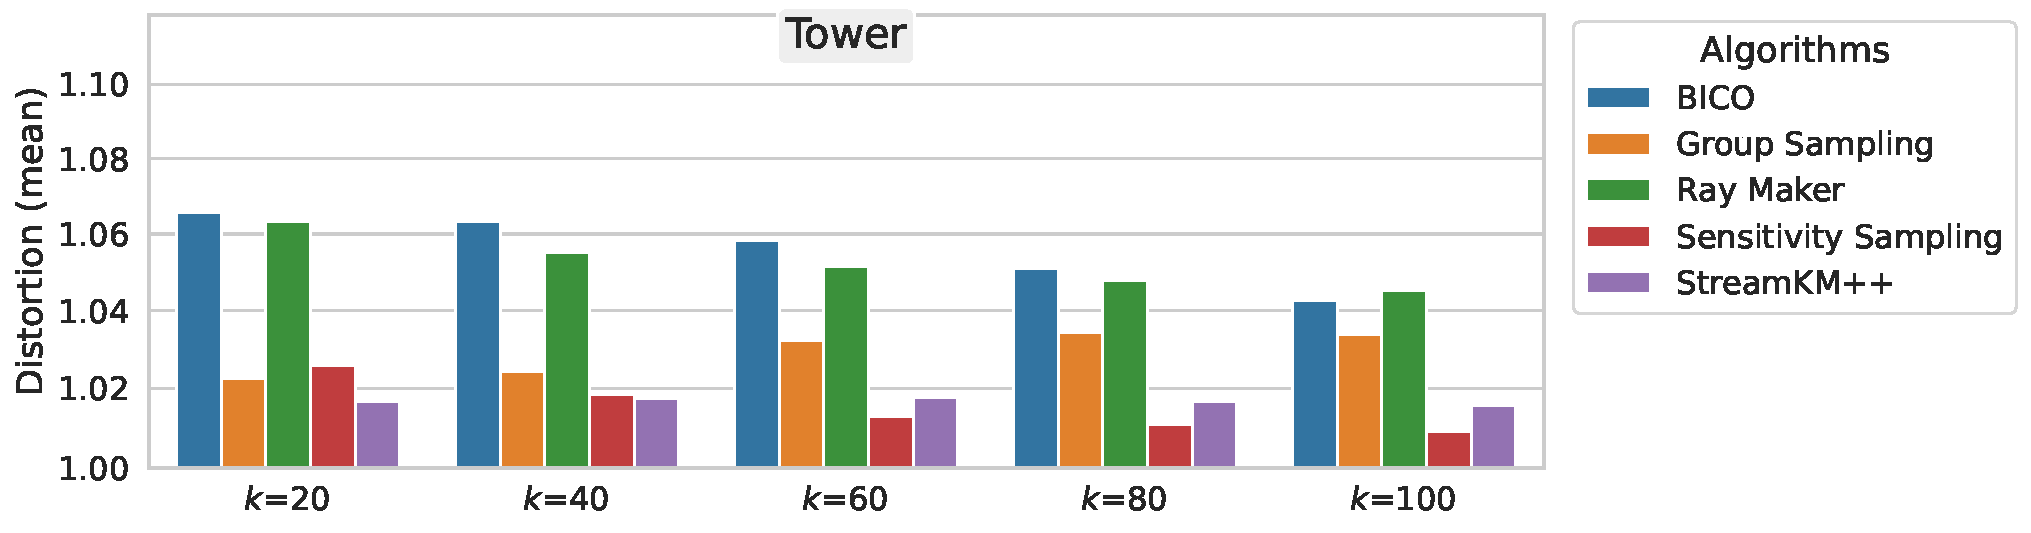
\includegraphics[width=.69\linewidth]{figures/distortions-mean-Tower.pdf}
  \newline \newline
  \subfloat{
    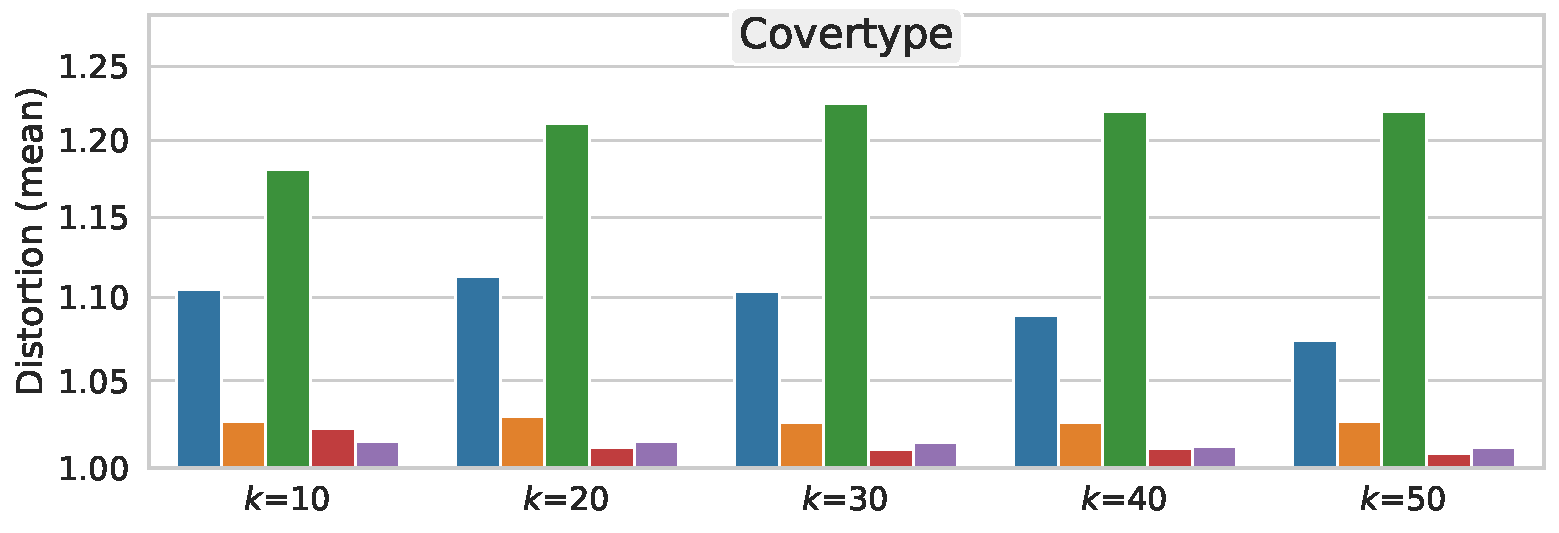
\includegraphics[width=0.5\textwidth]{figures/distortions-mean-Covertype.pdf}
  }
  \subfloat{
    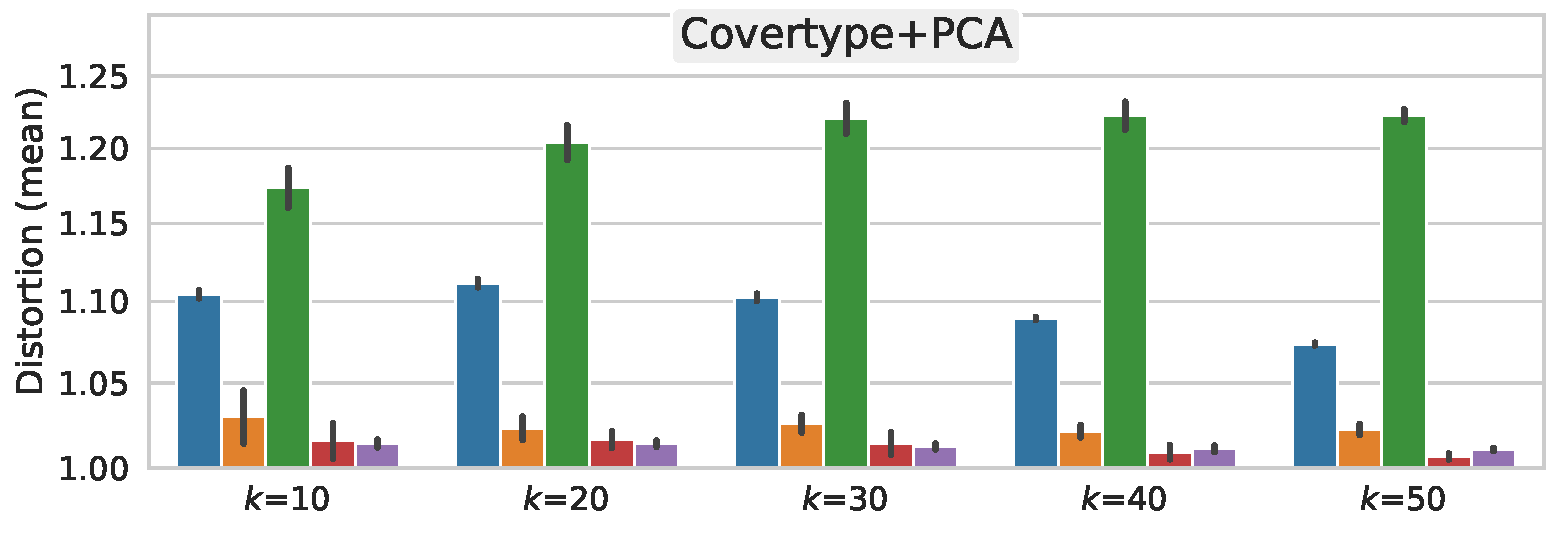
\includegraphics[width=.5\linewidth]{figures/distortions-mean-Covertype+PCA.pdf}
  }
  \newline \newline
  \subfloat{
    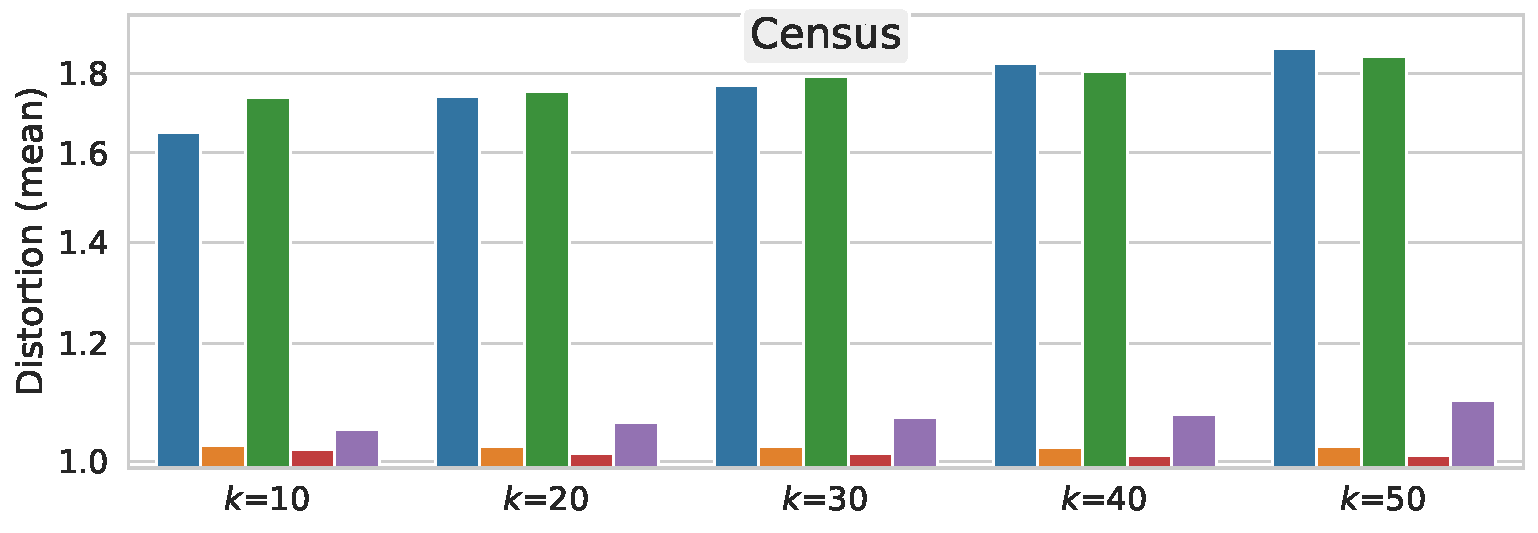
\includegraphics[width=0.5\textwidth]{figures/distortions-mean-Census.pdf}
  }
  \subfloat{
    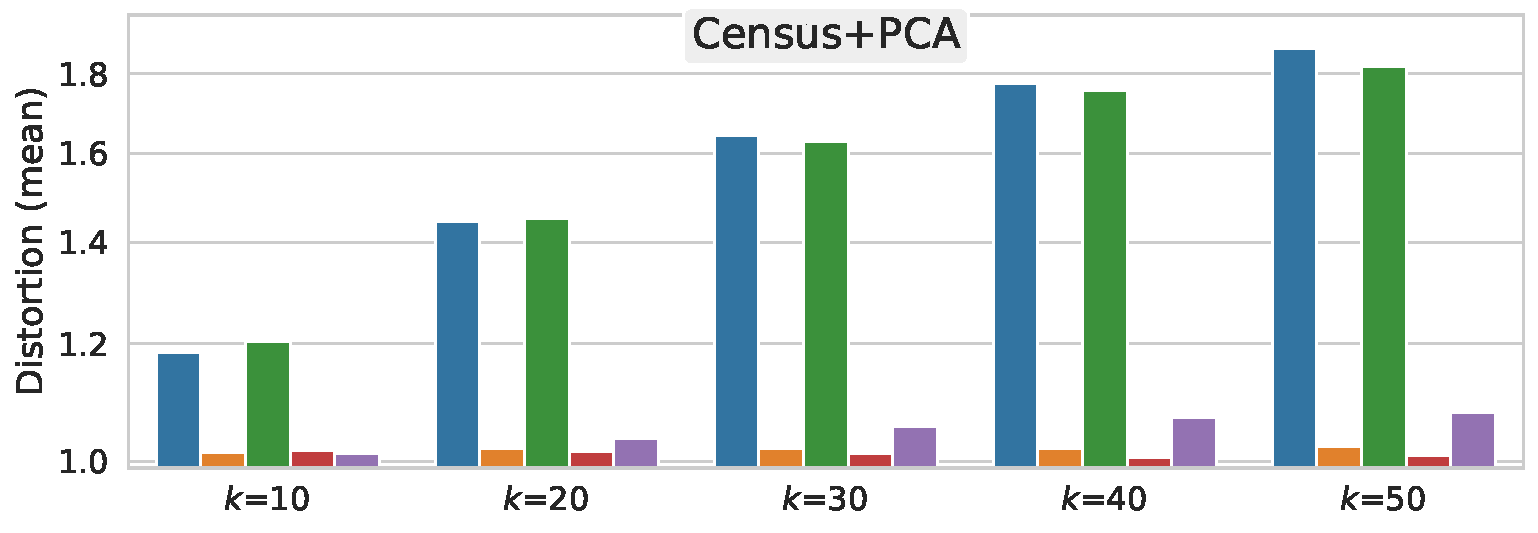
\includegraphics[width=.5\linewidth]{figures/distortions-mean-Census+PCA.pdf}
  }
  \newline \newline
  \subfloat{
    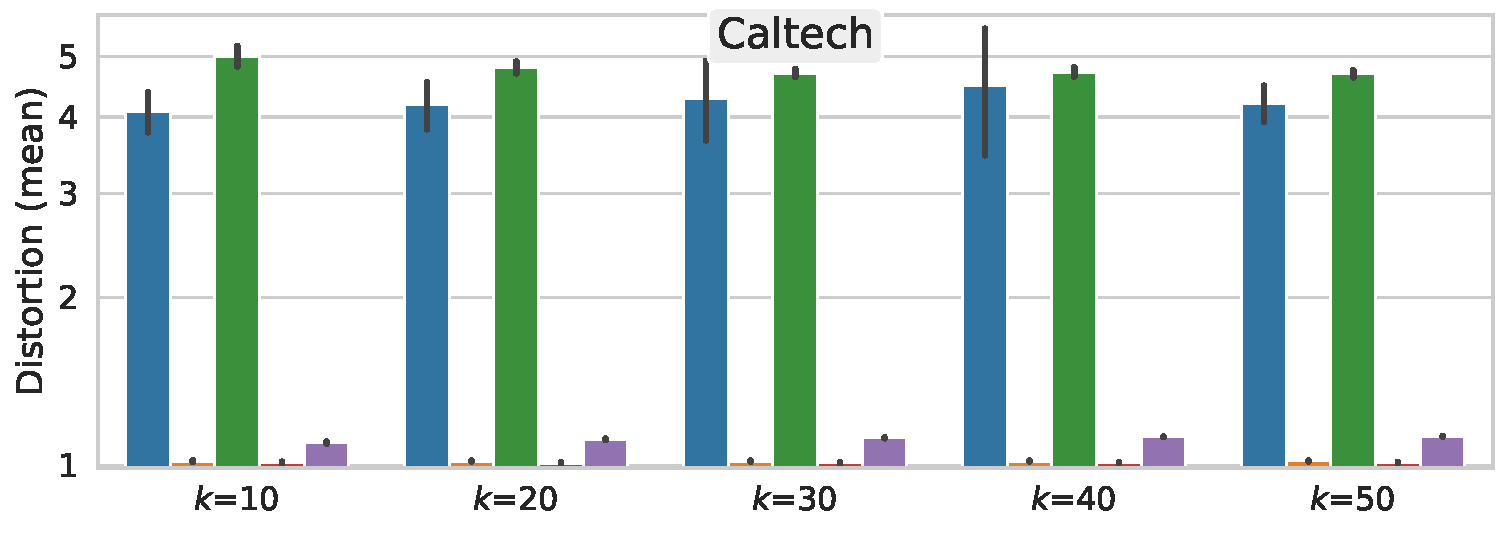
\includegraphics[width=0.5\textwidth]{figures/distortions-mean-Caltech.pdf}
  }
  \subfloat{
    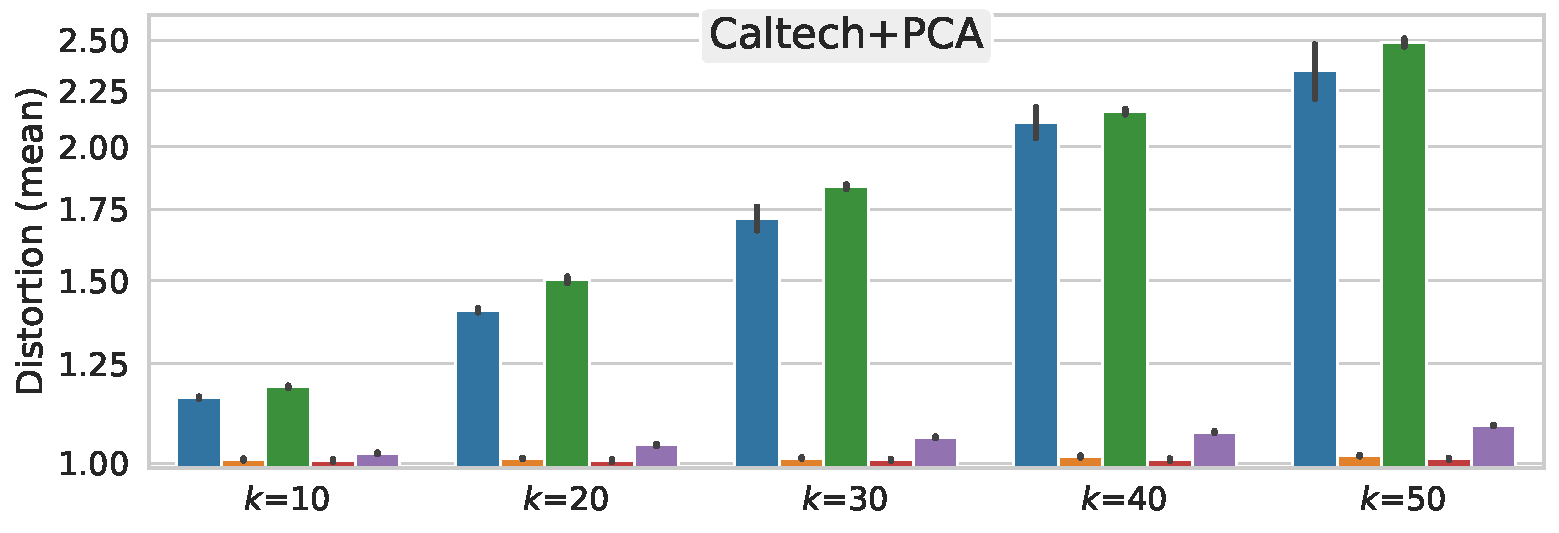
\includegraphics[width=.5\linewidth]{figures/distortions-mean-Caltech+PCA.pdf}
  }
  \newline \newline
  \subfloat{
    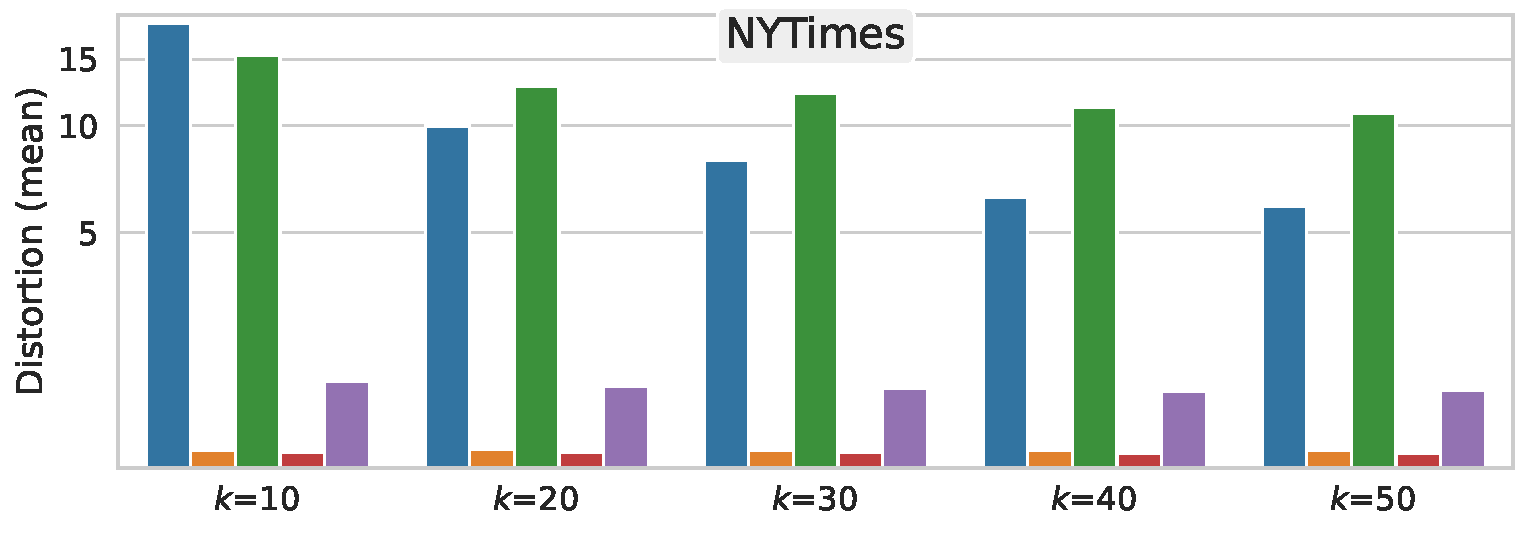
\includegraphics[width=0.5\textwidth]{figures/distortions-mean-NYTimes.pdf}
  }
  \subfloat{
    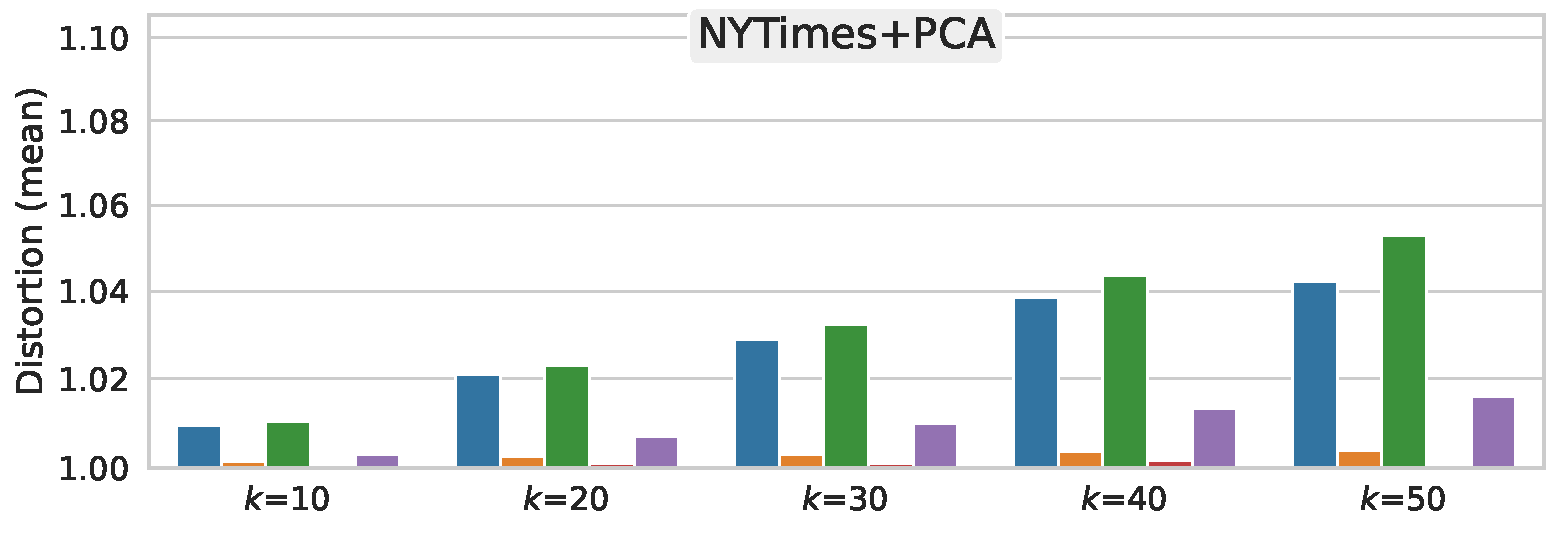
\includegraphics[width=.5\linewidth]{figures/distortions-mean-NYTimes+PCA.pdf}
  }
  \newline \newline
%   \subfloat{
%     \\[1ex]
%     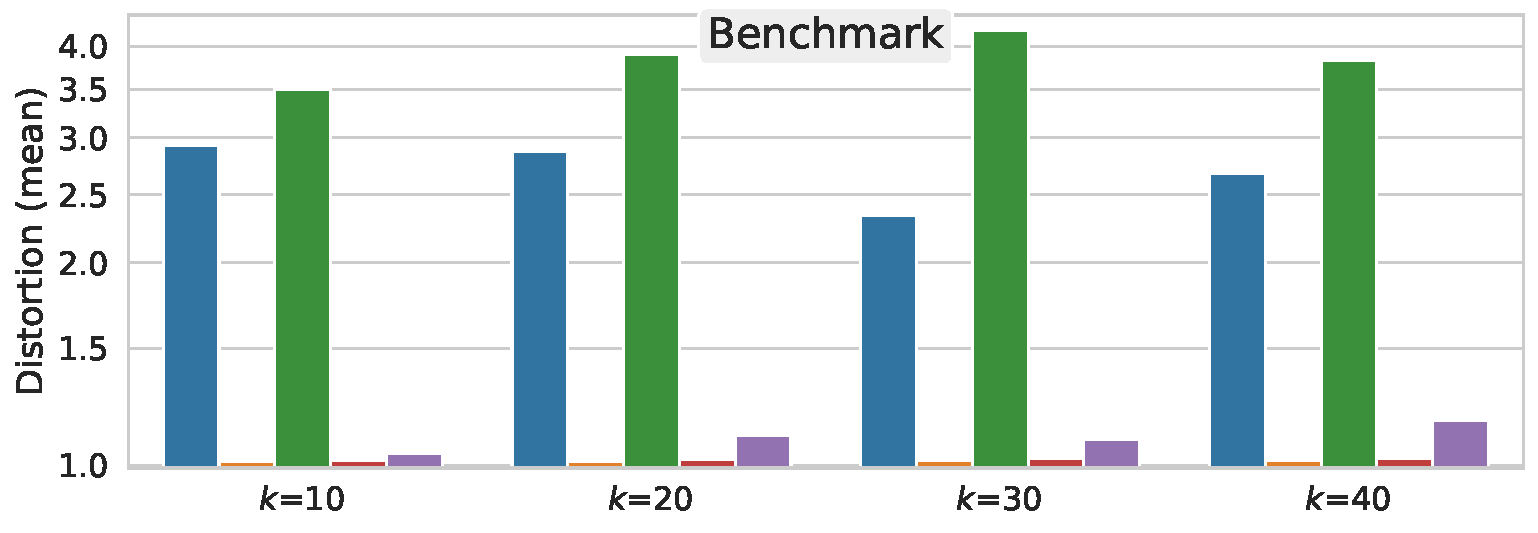
\includegraphics[width=0.5\textwidth]{figures/distortions-mean-Benchmark.pdf}
%   }
  \subfloat{
    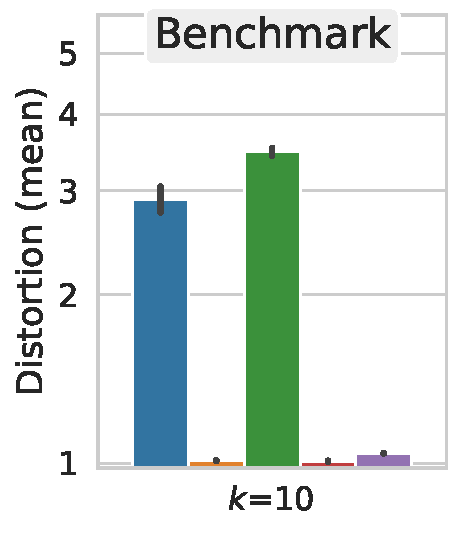
\includegraphics[width=0.165\textwidth]{figures/distortions-mean-Benchmark-k10.pdf}
    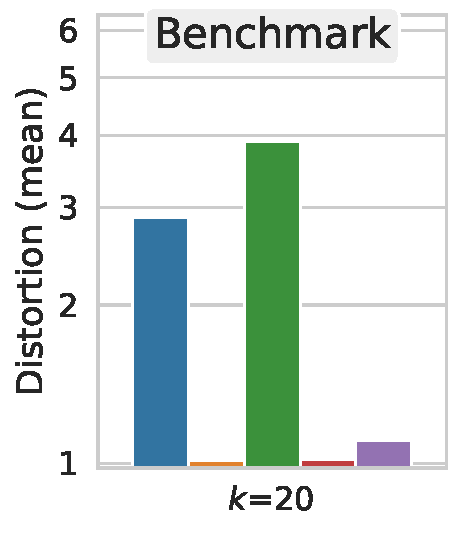
\includegraphics[width=0.165\textwidth]{figures/distortions-mean-Benchmark-k20.pdf}
    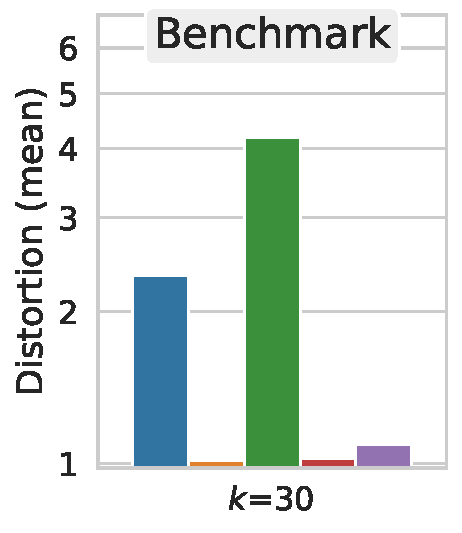
\includegraphics[width=0.165\textwidth]{figures/distortions-mean-Benchmark-k30.pdf}
    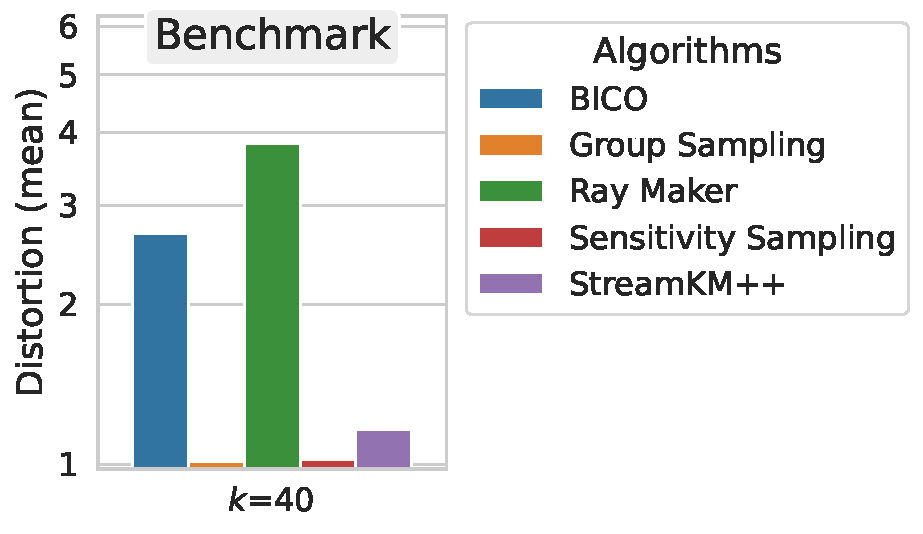
\includegraphics[width=0.331\textwidth]{figures/distortions-mean-Benchmark-k40.pdf}
  }
%   \subfloat{
%     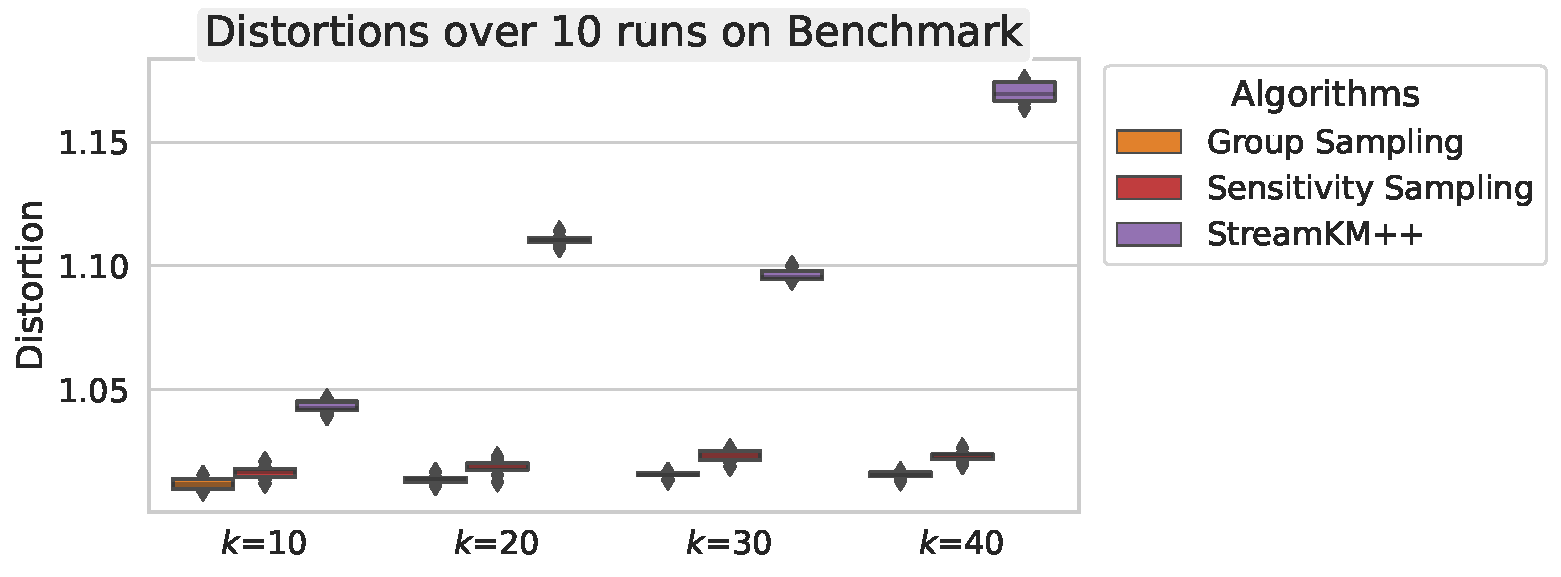
\includegraphics[width=.5\linewidth]{figures/boxplot-Benchmark-GS-SS-StreamKM.pdf}
%   }
  \caption{The distortions of the evaluated coreset algorithms with coreset size $T=200k$ on five real-world data sets and on four benchmark instances. Notice that the axis is non-linear as otherwise the bars for Sensitivity Sampling and Group Sampling would disappear on the plots as their distortions are close to 1.}
  \label{fig:distortions}
\end{figure*}







\subsection{Outcome of Experiments}
% We summarized the distortions for $T=200k$ in \cref{fig:distortions}.
We observed that in the majority of our experiments, varying the coreset sizes does not significantly change the performance profiles of individual algorithms when comparing them against each other. Therefore, in the following sections, we focus on a cross-section of the experiments where $m=200$ i.e., $T=200k$.
For numerical results including variances of all the experiments, we refer to \cref{sec:distortions-tables}. 

In~\cref{fig:distortions}, we summarized the distortions of the experiments with coreset sizes $T=200k$. All five algorithms are matched on the \textit{Tower} dataset. The worst distortions across the algorithms are close to 1, and performance between the algorithms is negligible. The performance difference between sampling-based and movement-based methods become more pronounced as the number of dimensions increase. On \textit{Covertype} with its 54 features, Ray Maker performs the worst followed by BICO and Group Sampling while Sensitivity Sampling and StreamKM++ perform the best. Differences in performance are more noticeable on \textit{Census}, \textit{Caltech}, and \textit{NYTimes}  where methods based on importance sampling perform much better. Sensitivity Sampling and Group Sampling perform the best, StreamKM++ come in second while BICO and Ray Maker perform the worst across these data sets.
On the \textit{Benchmark}, Ray Maker is the worst while Sensitivty Sampling and Group Sampling are the best. StreamKM++ performs also very well compared to BICO.

Reducing noise with PCA helped boost the performance on real-world data sets with large number of dimensions. On \textit{Covertype}, PCA does not change the performance numbers by much. On \textit{Census} ($d=68$), the preprocessing step with PCA improves the performance of BICO and Ray Maker slightly for lower values of $k$. The distortions of BICO and Ray Maker are reduced markedly on \textit{Caltech} ($d=128$) after applying PCA. 


\subsection{Interpretation of Experimental Results}



\subsubsection*{Optimization versus Compression}
While all five algorithms are equally matched when optimizing on the candidate coresets (see ~\cref{fig:real-costs}), coreset quality performance differ significantly (see \cref{fig:distortions}). 
% We omit tables and plots detailing the cost due to space restrictions. 
For all data sets, the obtained costs differed insignificantly for all values of $k$.

The quality of the coreset itself can be closely tied to the change in cost with increasing number of centers. It is not uncommon for the $k$-means cost of real-world data sets to drop significantly for larger values of $k$.
~\cref{fig:cost-curves-real-world-datasets} illustrates this behavior for several real-world data sets. The more the curve bends, the less of a difference there is between computing a coreset and a clustering with low cost. For data sets with a L-shaped cost curve, a coreset algorithm adding more centers to the coreset will seem to be performing well when evaluating it based on the outcome of the optimization.
\textit{Tower} is a good example of a data set where optimization is very close to compression. Its cost curve bends the most which indicates that adding more centers help reduce the cost. One of the strengths of the benchmark is that there is no way of reducing the cost without capturing the right subclusters within a benchmark instance. This means that the cost does not decrease markedly beyond a certain value of $k$ even if more centers are added, see~\cref{fig:cost-curves-benchmark} in the appendix. 

For BICO, Ray Maker, and StreamKM++, there is a correlation between the steepness of the cost curve for a data set and the distortion of the generated coreset. 
On data sets where the curve is less steep, we observed higher distortions. The effect is more pronounced for the movement-based algorithms (BICO and Ray Maker) than for StreamKM++. The other two sampling-based approaches (Group Sampling and Sensitivity Sampling) seem to be free from this behavior as they consistently generate high quality coresets irrespective of the shape of cost curve.







\begin{figure}
  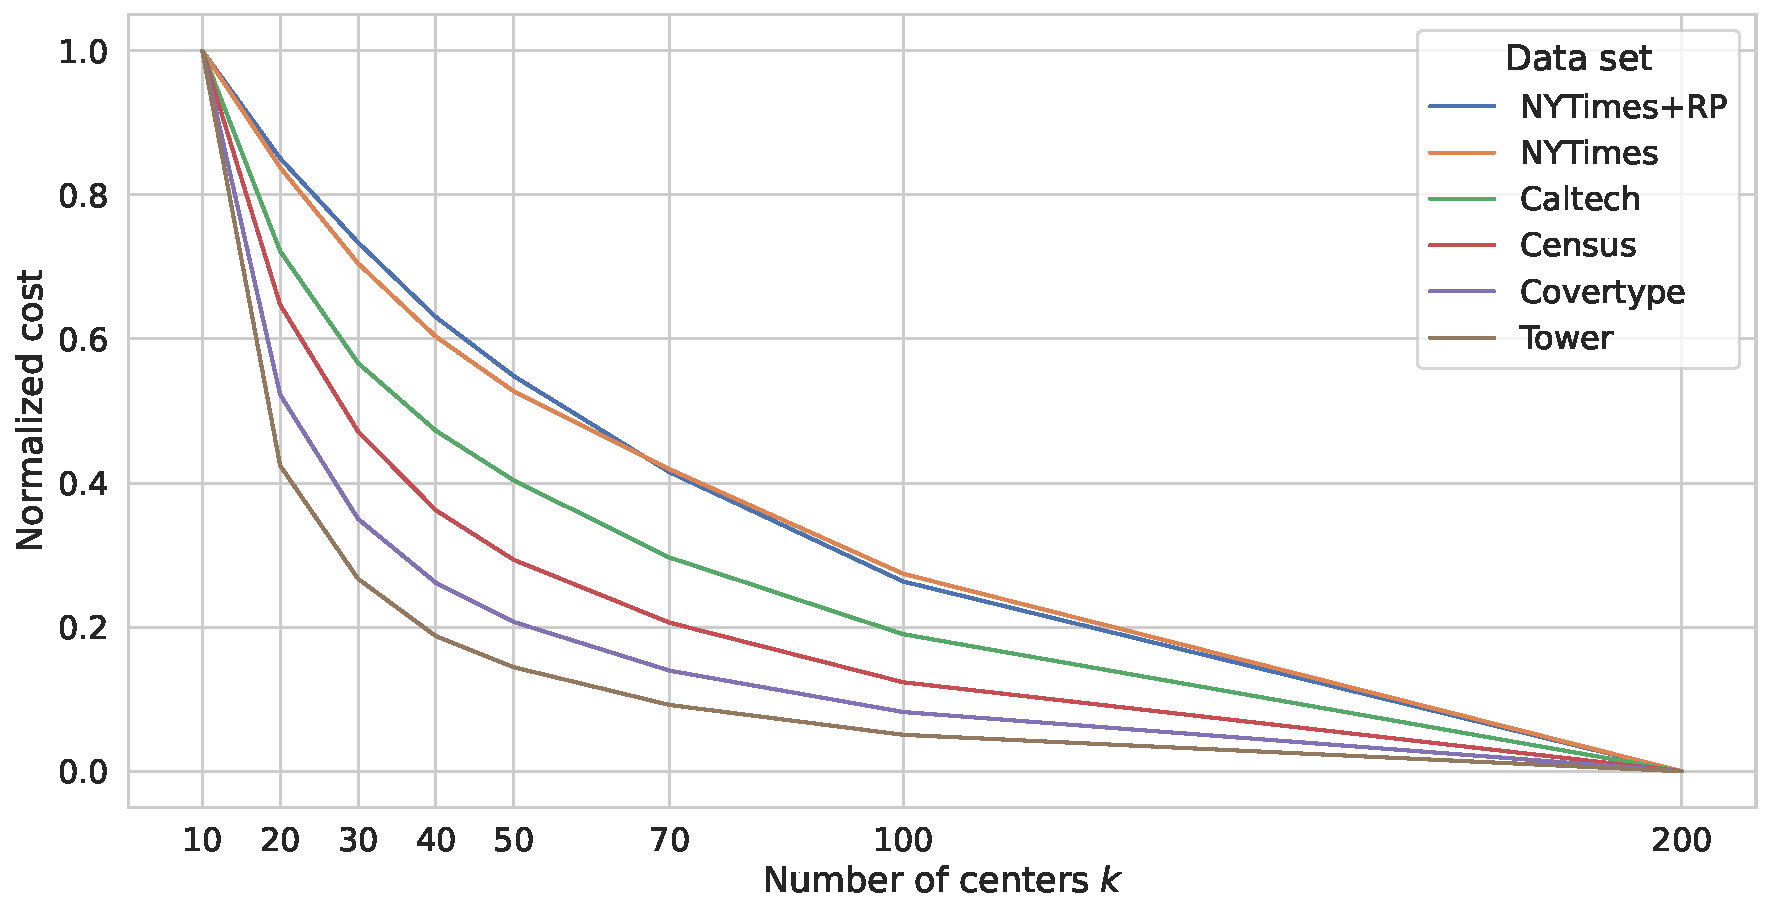
\includegraphics[width=1\linewidth]{figures/cost-curves-real-world-datasets.pdf}
  \caption{Depicts how clustering costs of five real-world data sets decrease as the number of centers increase. 
  % The most widely used data sets for evaluating coresets are \textit{Tower}, \textit{Covertype}, and \textit{Census}, while \textit{Caltech} is rarely used and \textit{NYTimes} has never been used before.
  Plotting the cost curve allows us to study whether we can observe a difference between coreset construction and optimization in a data set when evaluating a coreset based on cost.
  }
  \label{fig:cost-curves-real-world-datasets}
\end{figure}



\subsubsection*{Movement-based versus Sampling-based Approaches}

In general, movement-based constructions perform the worst in terms of coreset quality. 
We observed that BICO and Ray Maker have the highest distortions across all data sets including on the benchmark instances. Among the sampling-based algorithms, Sensitive Sampling performs well with Group Sampling generally being competitive. This runs contrary to theory where Group Sampling has the better (currently known) theoretical bounds. StreamKM++ is an interesting case. Like the movement-based methods, its distortion increases with the dimension. Nevertheless, it generally performs significantly better than BICO and Ray Maker. This can be attributed to the fact that the coreset produced by StreamKM++ consists entirely of $k$-means++ centers weighted by the number of points of a minimal cost assignment. This is similar to movement-based algorithms such as BICO. Nevertheless, it also retains some of the performance from pure importance schemes.

In practice as well as in theory, the distortion of movement-based algorithms are affected by the dimension. By comparison, sampling-based algorithms are affected very little. Theoretically, there should not exist a difference, as the sampling bounds are independent of the dimension. What little effect can be observed is likely due to PCA making it easier to find low cost solutions that form the backbone of all coreset constructions. StreamKM++ is an interesting case, as it is still affected by the dimension, though less than the other movement based methods, due its performance without dimension reduction being significantly better than the worst-case bounds would suggest. 





\subsubsection*{Impact of PCA}

On almost all our data sets, the performance improves when input data is preprocessed with PCA, especially for the movement-based algorithms. Empirically, the more noise is removed (i.e., small $k$ value), the lower the distortion. Notice that $k$ is the number of principal components that the input data is projected on to. The rest of the low variance components are treated as noise and removed. Method utilizing sampling (Group Sampling, Sensitivity Sampling and StreamKM++) are less effected by the preprocessing step. On \textit{Covertype}, PCA does not change the distortions by much because almost all the variance in the data is explained by the first five principal components (see~\cref{fig:explained-variance-pca}). 
On \textit{Caltech} and \textit{NYTimes}, the quality of the coresets by BICO and Ray Maker improves greatly because the noise removal is more aggressive. Even if the quality is much better for movement-based coreset constructions due to PCA, importance sampling methods are still superior when it comes to the quality of the compression. Summarizing, all methods benefit from PCA, and in case of movement based constructions, we consider PCA a necessary preprocessing step. For the sampling based methods, the computational expense of using PCA in preprocessing does not seem justify the comparatively meagre gains in coreset distortion.


